%===================================================================================
% JORNADA CIENTÍFICA ESTUDIANTIL - MATCOM, UH
%===================================================================================
% Esta plantilla ha sido diseñada para ser usada en los artículos de la
% Jornada Científica Estudiantil de MatCom.
%
% Por favor, siga las instrucciones de esta plantilla y rellene en las secciones
% correspondientes.
%
% NOTA: Necesitará el archivo 'jcematcom.sty' en la misma carpeta donde esté este
%       archivo para poder utilizar esta plantila.
%===================================================================================



%===================================================================================
% PREÁMBULO
%-----------------------------------------------------------------------------------
\documentclass[a4paper,10pt,twocolumn]{article}

%===================================================================================
% Paquetes
%-----------------------------------------------------------------------------------
\usepackage{amsmath}
\usepackage{amsfonts}
\usepackage{graphicx}
\usepackage{amssymb}
\usepackage{jcematcom}
\usepackage[utf8]{inputenc}
\usepackage{listings}
\usepackage[pdftex]{hyperref}
\usepackage{caption}
\usepackage{xcolor}
\usepackage{subcaption}
\usepackage[hidelinks]{hyperref}
%-----------------------------------------------------------------------------------
% Configuración
%-----------------------------------------------------------------------------------
\hypersetup{colorlinks,%
	    citecolor=black,%
	    filecolor=black,%
	    linkcolor=black,%
	    urlcolor=blue}
\definecolor{codegreen}{rgb}{0,0.6,0}
\definecolor{codegray}{rgb}{0.5,0.5,0.5}
\definecolor{codepurple}{rgb}{0.58,0,0.82}
\definecolor{backcolour}{rgb}{0.95,0.95,0.92}
\definecolor{crimson}{HTML}{DC1420}
\definecolor{customGreen}{HTML}{228B22}
\definecolor{marron}{HTML}{804000}
\definecolor{orange}{HTML}{FFA500}
\lstdefinestyle{mystyle}{
			backgroundcolor=\color{backcolour},   
			commentstyle=\color{codegreen},
			keywordstyle=\color{magenta},
			numberstyle=\tiny\color{codegray},
			stringstyle=\color{codepurple},
			basicstyle=\ttfamily\footnotesize,
			breakatwhitespace=false,         
			breaklines=true,                 
			captionpos=b,                    
			keepspaces=true,                 
			numbers=left,                    
			numbersep=5pt,                  
			showspaces=false,                
			showstringspaces=false,
			showtabs=false,                  
			tabsize=2
		}
\lstset{keepspaces=true, style=mystyle}

%===================================================================================



%===================================================================================
% Presentacion
%-----------------------------------------------------------------------------------
% Título
%-----------------------------------------------------------------------------------
\title{Modelo de análisis predictivo del crecimiento poblacional: Estimación de la capacidad de carga}


%-----------------------------------------------------------------------------------
% Autores
%-----------------------------------------------------------------------------------
\author{\\
\name Guillermo Cepero Garcia \email \href{mailto:thewillyjake53@gmail.com}{thewillyjake53@gmail.com}
	\\ \addr Grupo D111 \AND
\name Luis Ernesto Serras Rimada \email \href{mailto:luisernestoserras@gmail.com}{luisernestoserras@gmail.com}
  \\ \addr Grupo D111 \AND
\name Miguel Vadim Vilarino Pedraza \email \href{mailto:miguelvadim04@gmail.com}{miguelvadim04@gmail.com}
	\\ \addr Grupo D111}



%-----------------------------------------------------------------------------------
% Tutores
%-----------------------------------------------------------------------------------
\tutors{\\
Dr. Tutor Uno, \emph{Centro} \\
Lic. Tutor Dos, \emph{Centro}}

%-----------------------------------------------------------------------------------
% Headings
%-----------------------------------------------------------------------------------
\jcematcomheading{\the\year}{1-\pageref{end}}{A. Uno, A. Dos}

%-----------------------------------------------------------------------------------
\ShortHeadings{Modelo predictivo del crecimiento poblacional}{Autores}
%===================================================================================



%===================================================================================
% DOCUMENTO
%-----------------------------------------------------------------------------------
\begin{document}

%-----------------------------------------------------------------------------------
% NO BORRAR ESTA LINEA!
%-----------------------------------------------------------------------------------
\twocolumn[
%-----------------------------------------------------------------------------------

\maketitle

%===================================================================================
% Resumen y Abstract
%-----------------------------------------------------------------------------------
\selectlanguage{spanish} % Para producir el documento en Español

%-----------------------------------------------------------------------------------
% Resumen en Español
%-----------------------------------------------------------------------------------
\begin{abstract}

	El análisis del crecimiento poblacional reviste gran importancia debido a su relevancia en diversos campos como la economía, demografía, epidemiología y la ecología. Resulta útil en múltiples ámbitos, incluyendo estudios demográficos, planificación urbana y análisis de recursos naturales. Conocer un resultado aproximado que se acerque a una solución real del crecimiento poblacional permitiría beneficiar significativamente la dirección y gestión de recursos en nuestro país. Los resultados obtenidos en el análisis demuestran la importancia de adaptar modelos matemáticos a patrones de crecimiento reales complejos, considerando factores como la heterogeneidad temporal en los datos y la posibilidad de cambios abruptos en las tasas de crecimiento. La comparación entre diferentes modelos, como el modelo logístico tradicional versus uno ajustado, proporciona valiosas lecciones sobre cómo mejorar la precisión de las predicciones demográficas. Se observó que el segundo modelo, con intervalos de 8 años, se ajustaba mejor, reflejando valores cercanos a la densidad poblacional promedio. Además, se identificaron problemas en las respuestas de los parámetros estimados dentro de ciertos intervalos, atribuidos a una tendencia casi vertical en los valores durante ciertos periodos. Esto llevó a proponer un ajuste diferente al utilizado con todos los datos, basado en un crecimiento más acelerado. En los años 1980 en adelante, Cuba experimentó un crecimiento poblacional significativo, seguido de un período de estabilización y eventual disminución de la tasa de crecimiento. Este análisis demuestra la necesidad de considerar factores específicos del contexto cubano, como el impacto de eventos históricos en el patrón de crecimiento poblacional.

\end{abstract}

%-----------------------------------------------------------------------------------
% English Abstract
%-----------------------------------------------------------------------------------
\vspace{0.5cm}

\begin{enabstract}

	The analysis of population growth is of great importance due to its relevance in various fields such as economics, demography, epidemiology and ecology. It is useful in multiple areas, including demographic studies, urban planning and natural resource analysis. Knowing an approximate result that is close to a real solution to population growth would significantly benefit the direction and management of resources in our country. The results obtained in the analysis demonstrate the importance of adapting mathematical models to complex real growth patterns, considering factors such as temporal heterogeneity in the data and the possibility of abrupt changes in growth rates. Comparison between different models, such as the traditional logistic model versus an adjusted one, provides valuable lessons on how to improve the accuracy of demographic predictions. It was observed that the second model, with intervals of 8 years, fit better, reflecting values ​​close to the average population density. In addition, problems were identified in the responses of the estimated parameters within certain intervals, attributed to an almost vertical trend in the values ​​during certain periods. This led to proposing a different adjustment than that used with all the data, based on more accelerated growth. In the 1980s onwards, Cuba experienced significant population growth, followed by a period of stabilization and eventual decline in the growth rate. This analysis demonstrates the need to consider factors specific to the Cuban context, such as the impact of historical events on the population growth pattern.
\end{enabstract}

%-----------------------------------------------------------------------------------
% Palabras clave
%-----------------------------------------------------------------------------------
\begin{keywords}
	Predicción,
	carga,
	poblacion,
	datos,
	modelo,
	entrenamiento,
	capacidad.
\end{keywords}

%-----------------------------------------------------------------------------------
% Temas
%-----------------------------------------------------------------------------------
\begin{topics}
	Predicción de crecimiento poblacional, estimación del valor de la capacidad de carga.
\end{topics}


%-----------------------------------------------------------------------------------
% NO BORRAR ESTAS LINEAS!
%-----------------------------------------------------------------------------------
\vspace{0.8cm}
]
%-----------------------------------------------------------------------------------


%===================================================================================

%===================================================================================
% Introducción
%-----------------------------------------------------------------------------------
\section{Introducción}\label{sec:intro}
%-----------------------------------------------------------------------------------
El crecimiento poblacional es un fenómeno global que ha tenido un impacto significativo en el desarrollo económico y social de los países. Según las proyecciones de la Organización de las Naciones Unidas para el Desarrollo (ONU), la población mundial alcanzó los 7.9 mil millones en 2021 y se espera que llegue a 9.7 mil millones en 2050 y 11.2 mil millones en 2021$^{1}$. Este crecimiento demográfico tiene implicaciones tanto positivas como negativas para el desarrollo sostenible. Por un lado, el aumento de la población puede generar impulso económico y laboral, especialmente en países con economías en desarrollo. Sin embargo, también plantea desafíos significativos en términos de infraestructura urbana, recursos naturales y servicios públicos\\
La variación histórica de la población en Cuba ha sido notable. Según datos del Instituto Nacional de Estadísticas de Cuba, la población del país aumentó de aproximadamente 6.5 millones en 1953 hasta alcanzar un máximo de 11.2 millones en 2016. Desde entonces, ha experimentado una ligera disminución, llegando a los 11.0 millones en 2022$^{2}$. Las causas principales de este patrón de crecimiento han incluido factores como la política socialista de Cuba (que priorizó la educación y la salud pública, lo que llevó a un aumento en la esperanza de vida y la reducción de la mortalidad infantil); las migraciones internacionales (especialmente desde la década de 1990); los cambios en las políticas familiares, como la legalización del aborto y la anticoncepción, que afectaron la fertilidad de la población y el impacto de la crisis económica de 1991, que llevó a un cambio en las actitudes hacia la planificación familiar; entre otros. Es importante destacar que el análisis del crecimiento poblacional debe considerar no solo estos factores, sino también sus impactos socioeconómicos y ambientales. Por ejemplo, el rápido crecimiento urbano en muchas ciudades cubanas ha generado desafíos en términos de infraestructura urbana y servicios públicos$^{2}$\\
Por tanto, los objetivos principales al realizar un análisis del crecimiento poblacional mediante la estimación de la capacidad de carga poblacional son: 
\begin{itemize}
	\item Estimar el número máximo de personas que pueden ser sostenidamente alojadas en un área geográfica determinada y evaluar el equilibrio entre la población existente y la capacidad de carga ambiental, lo que puede contribuir a determinar si una región ha alcanzado o excedido su capacidad de carga, permitiendo tomar decisiones informadas sobre planeamiento urbano, desarrollo económico y políticas de control de natalidad. 
	\item Contribuir al diseño de estrategias de planificación urbana y rural que equilibren el crecimiento económico con la protección del medio ambiente y los servicios básicos. 
	\item Permitir evaluar el impacto potencial del cambio climático y otros factores externos en la capacidad de carga poblacional a largo plazo. 
	\item Contribuir al diseño de programas de educación ambiental y concientización sobre las implicaciones del crecimiento poblacional.
	\item Y ayudar a establecer límites razonables para el crecimiento demográfico, evitando excederse en la explotación de recursos naturales y servicios públicos. 
\end{itemize}

%===================================================================================



%===================================================================================
% Desarrollo
%-----------------------------------------------------------------------------------
\section{Modelo Matemático}\label{sec:dev}
%-----------------------------------------------------------------------------------
 Se plantea trabajar el asunto con un modelo matemático que nos pueda conducir a dicha prediccion, y se considera 
 el \textbf{modelo del crecimiento logístico}$^{3}$, que es solución de la ecuación diferencial que describe cómo la tasa de crecimiento de la población (dP/dt) 
 cambia con el tamaño de la población (P(t)). Cuando la población es pequeña, la tasa de crecimiento es alta, ya que 
 hay muchos recursos disponibles para cada individuo. A medida que la población crece, la tasa de crecimiento disminuye 
 porque hay menos recursos disponibles por individuo. Cuando la población alcanza su capacidad de carga (K), la tasa 
 de crecimiento se vuelve cero, indicando que la población ha alcanzado un equilibrio sostenible.\\
 Entonces se tiene que:
\begin{itemize}
    \item (P(t)) es la población en función del tiempo (t).
    \item (r) es la tasa de crecimiento intríseca de la población.
    \item (K) es la capacidad de carga o tamaño máximo sostenible de la población.
\end{itemize}\\
\underline{Parámetros a Estimar:}
\begin{itemize}
    \item (r): Tasa de crecimiento  de la población. 
    \item (K): Capacidad de carga de la población.
\end{itemize}\\
\textbf{\underline{Ecuacion Diferencial de Modelo Logístico:}} $\frac{dP}{dt} = r \cdot P(t)(1 - \frac{P(t)}{K}) $\\\\

Para obtener la capacidad de carga de la población cubana siguiendo el contexto del modelo logístico y utilizando 
datos reales, se debe seguir un proceso que involucre la recopilación de datos sobre la población cubana y 
los factores que podrían influir en su capacidad de carga. Estos pueden incluir la disponibilidad de recursos 
naturales, la infraestructura, la salud pública, y la economía.\\
Y posteriormente el análisis de esos datos y la interpretación de los resultados(Analisis Exploratorio).\\
Por ejemplo, supongamos que después de nuestro análisis, encontramos que la tasa de crecimiento intríseca (r) de la población 
cubana es de 0.02 (un 2\% anual) y que la capacidad de carga (K) estimada es de 15 millones de habitantes. 
Esto significaria que, teóricamente, nuestro país podría soportar hasta 15 millones de personas sin agotar sus recursos 
vitales, siempre y cuando se mantengan las condiciones actuales y se gestionen adecuadamente los recursos.\\
Como idea de solución se propone este modelo, el cual describe cómo la población crece hacia su capacidad de 
carga y luego se estabiliza.\\ 
\underline{La función logística tiene la forma:} $P(t) = \frac{K}{1 + Ae^{-rt}}$ $^{4}$\\
Donde (A) es una constante que depende de las condiciones iniciales de la población. Esta función muestra claramente 
el punto de inflexión, donde la tasa de crecimiento cambia de positiva a negativa, indicando que la población 
ha alcanzado su capacidad de carga y está comenzando a estabilizarse.
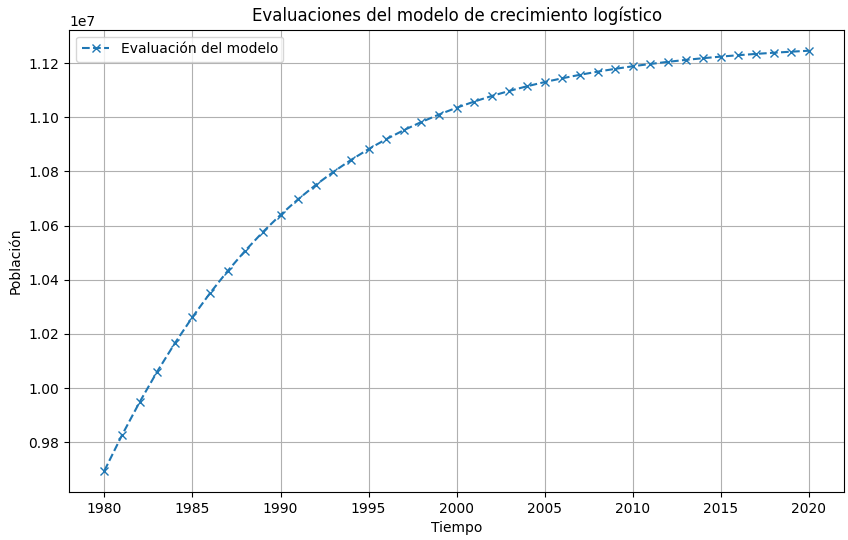
\includegraphics[width=0.45\textwidth]{img/model.png}$^{5}$\\
Para encontrar (A), se requiere conocer el valor inicial de la población, (P(0)), y usarlo junto con (K) y (r) 
para resolver (A). La condición inicial (P(0)) te da el valor de la población en el momento inicial, antes de 
que comience el crecimiento logístico.\\
\underline{La ecuación para encontrar (A) es:} $P(0) = \frac{K}{1 + Ae^{0}}$\\
Resolviendo para (A), obtenemos: $A = \frac{K}{P(0)} - 1$\\
Una vez que se tenga el valor de (A), se puede sustituir en la solución general de la ecuación diferencial 
logística para obtener la función que describe el crecimiento de la población hacia su capacidad de carga.
Por ejemplo, si se sabe que la población inicial es de 1000 individuos (P(0) = 1000), la capacidad de carga 
es de 10,000 individuos ((K = 10,000)), y la tasa de crecimiento es de 0.01 ((r = 0.01)), 
se puede calcular (A) de la siguiente manera:\\
$A = \frac{10,000}{1000} - 1 = 9$\\
Luego, se puede sustituir (A = 9) en la solución general para obtener la función específica que describe cómo la 
población crecerá hacia su capacidad de carga máxima.\\\\

%-----------------------------------------------------------------------------------
	\subsection{Modelo numérico}\label{sub:num}
%-----------------------------------------------------------------------------------
Se utilizaron los datos$^{6}$ históricos de densidad poblacional desde 1980 hasta 2020 publicados en las series estadísticas del sitio web de la Oficina Nacional de Estadissticas e Informacion (ONEI)$^{7}$. Y se desean ajustar los parámetros de la capacidad de carga($K$) y la tasa ($r$).
Para ello se decide utilizar la aproximación por mínimos cuadrados por medio de la función curvefit del módulo scipy.optimize en Python, cuya función matemáticamente se puede representar como:\\
Minimizar: $\sum_{i=1}^{N} (y_{i} - f(x_{i}, \theta))^2 $ \\
Donde toma los parámetros:
\begin{itemize}
	\item f: es la función modelo para la optimización.
	\item xdata: son los valores independientes (el tiempo ($t$ como $x_{i}$)).
	\item ydata: son los valores dependientes (los valores de densidad poblacional en función del tiempo ($P$ como $y_{i}$)).
	\item p0: Estimación inicial.$^{8}$
\end{itemize}
Y procede de la forma:\\ $$min[\sum_{i=1}^{N} (P(t_{i}) - (\frac{K}{1+\frac{K}{(P(0)-1)}e^{-rt_{i}}}))^{2}]^{\frac{1}{2}}$$
La función curvefit intentará minimizar la suma de los cuadrados de los residuales para encontrar los valores óptimos de $K$ y $r$ que minimizan esta expresión. 


%-----------------------------------------------------------------------------------
	\subsection{Implementación en Python}\label{sub:python}
%-----------------------------------------------------------------------------------
Se propone el desarrollo por medio de dos modelos diferentes, uno sin intervalos y otro con iteraciones por intervalos\\
Primero se define la función logística sin intervalos.
% Configuración de Listings
\lstset{keywordstyle=\color{blue}, basicstyle=\small}
\begin{lstlisting}[language=Python, caption=Código función logística sin intervalos]
def gen_log(p0):
	def logistic_function(t, K, r):
		return K / (1 + (K/p0 - 1) * np.exp(-r * t))
	return logistic_function
				
f = gen_log(P_data[0])
\end{lstlisting}

La siguiente celda de código ajustará la función logística a los datos observados, buscando los valores óptimos de $(K)$ y $(r)$ que minimicen la diferencia entre los datos observados y los predichos por el modelo.\\ 
Observaciones:
\begin{itemize}
	\item La función \textbf{`curvefit`} del módulo \textbf{`scipy.optimize`} devuelve dos arrays: \textbf{`popt`}, que contiene los \textbf{parámetros estimados} , y `pcov`, que contiene la \textbf{covarianza de los parámetros estimados}.
	\item La función \textbf{`curvefit`} es parte de la biblioteca \textbf{`SciPy`} y se utiliza para ajustar una función a un conjunto de datos mediante el método de \textbf{mínimos cuadrados}. Su objetivo principal es encontrar los parámetros de la función que minimizan la diferencia entre los valores observados y los predichos por la función.
\end{itemize}

\lstset{keywordstyle=\color{blue}, basicstyle=\small}
\begin{lstlisting}[language=Python, caption=Estimación de parámetros con la función sin intervalos]
# Parámetros iniciales:
initial_guess = [10000000, 0.01]  # Asume un valor inicial para K y r

# Ajustar el modelo a los datos observados
popt, pcov = curve_fit(f, t_data, P_data, p0=initial_guess, sigma=None, absolute_sigma=False)

# Imprimir los parámetros estimados
print("Parámetros estimados:", popt)
#Se formatean los datos:
params_formateados = [format(param, ".2f") for param in popt]
print("Parametros formateados: \n", params_formateados)

#Asignacion:
K = float(params_formateados[0])
K = int(K) #Parametro K
r_intr = float(params_formateados[1]) # Tasa intrinseca de crecimiento r
df_sin_intervalos = DataFrame({"K":K, 
                               "r":r_intr}, index=[0])
\end{lstlisting}
De este modelo inicial lo que se obtuvo como resultado al evaluar fueron valores muy cercanos a la línea real de los datos que se tiene, pero lógicamente no conviene para intentar realizar una predicción exacta para años posteriores.\\
Por tanto, acto seguido: se procede a desarrollar un segundo modelo para grupos de intervalos de 5, 8 y 10 años

\lstset{keywordstyle=\color{blue}, basicstyle=\small}
\begin{lstlisting}[language=Python, caption=Estimación de parámetros de la función con intervalos]
initial_guess = [10000000, 0.01]
def model(t, P, times):
    results = {}
    def estimate(times):
        x = 0
        y = times
        estimate_k = []
        estimate_r=[]
        estimate_lenght = int((n-3)/times)
        for _ in range(estimate_lenght):
            par_t = t[x:y]
            par_P = P[x:y]
            f = gen_log(par_P[0]) 
            # Ajustar el modelo a los datos observados
            popt, pcov = curve_fit(f, par_t, par_P, p0=initial_guess, sigma=None, absolute_sigma=False)
            params_formateados = [format(param, ".2f") for param in popt]
            popt_formateado = list(map(lambda x: float(x), popt))
            estimate_k.append(popt_formateado[0])
            estimate_r.append(popt_formateado[1])
            x += times
            y += times
        return [int(x) for x in estimate_k], [np.round(x,3) for x in estimate_r], pcov
    for i in times:
        K, r, cov = estimate(i)
        results[str(i) + " años"] = {"K": K, "r" : r, "Covarianza" : cov}
    return results
#Llamada a la función del modelo por intervalos
results = model(t_data[:-3], P_data[:-3], [5,8,10])
\end{lstlisting}

De los resultados se pueden identificar varios problemas en las respuestas de los parámetros estimados dentro de ciertos intervalos para cada rango. Esta situación se debe a que los valores en esos periodos presentan una tendencia casi vertical, caracterizada por una inclinación pronunciada hacia arriba. Como resultado, el valor de K podría verse afectado, ya que teóricamente, cuando el tiempo tiende a infinito, la función poblacional tiende a K. En consecuencia, en la primera aproximación global, K proporciona un valor cercano a la población total de Cuba (11 millones).\\

Es importante tener en cuenta que los datos reales no siguen exactamente la curva logística ideal. La función real presenta segmentos más concavos y otros más convexos que la función teórica. Por esta razón, se realizará un ajuste diferente al utilizado con todos los datos, basándose en un crecimiento más acelerado. Este ajuste se justifica porque los puntos en cuestión muestran una tendencia más vertical, lo que implica aumentos significativos en la población. Dado que estos aumentos son tan pronunciados, es razonable esperar que K también experimente una subida considerable.\\
Con respecto a los resultados de la evaluación de predicción se tuvo que el segundo modelo (intervalos de 8 años) fue el que mejor se ajustó y al representarlo se reflejaron valores bastante cercanos a la densidad poblacional promedio lo que indica un correcto ajuste.\\

Por otro lado cabe resaltar que en los años 1980 en adelante la isla experimentó un crecimiento poblacional significativo, pero luego se comenzó a establizar y eventualmente disminuir.


%===================================================================================


%===================================================================================
% Conclusiones
%-----------------------------------------------------------------------------------
\section{Conclusiones}\label{sec:conc}
El análisis de los resultados reveló varios dificultades, las cuales se deben principalmente a la presencia de una tendencia casi vertical en los valores durante ciertos periodos, caracterizada por una inclinación pronunciada hacia arriba.\\
Primeramente se visualiza una comparación de valores reales vs estimaciones del modelo sin intervalos para las estimaciones de ['11280122.85', '0.10'] devueltas por la función utilizada.
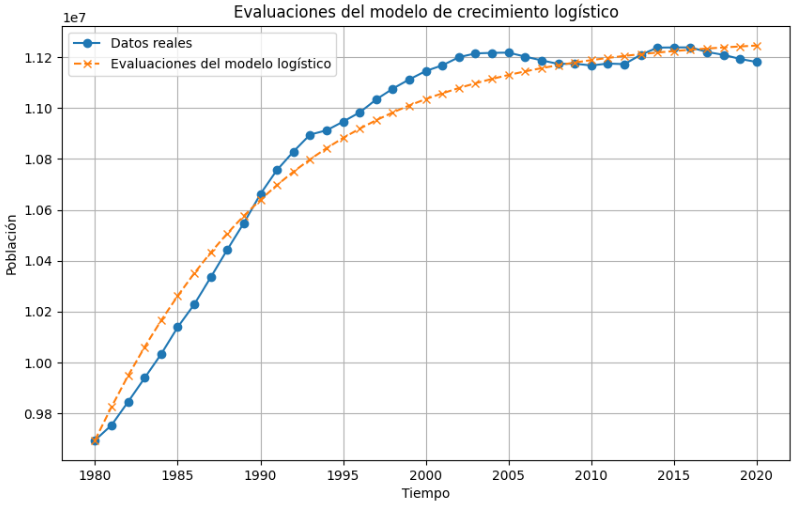
\includegraphics[width=0.45\textwidth]{img/real_vs_pred.png}
Donde se alcanza a apreciar un ajuste muy acertado.\\ 
Luego, para una prediccion utilizando las mismas estimaciones para años anteriores se obtiene:
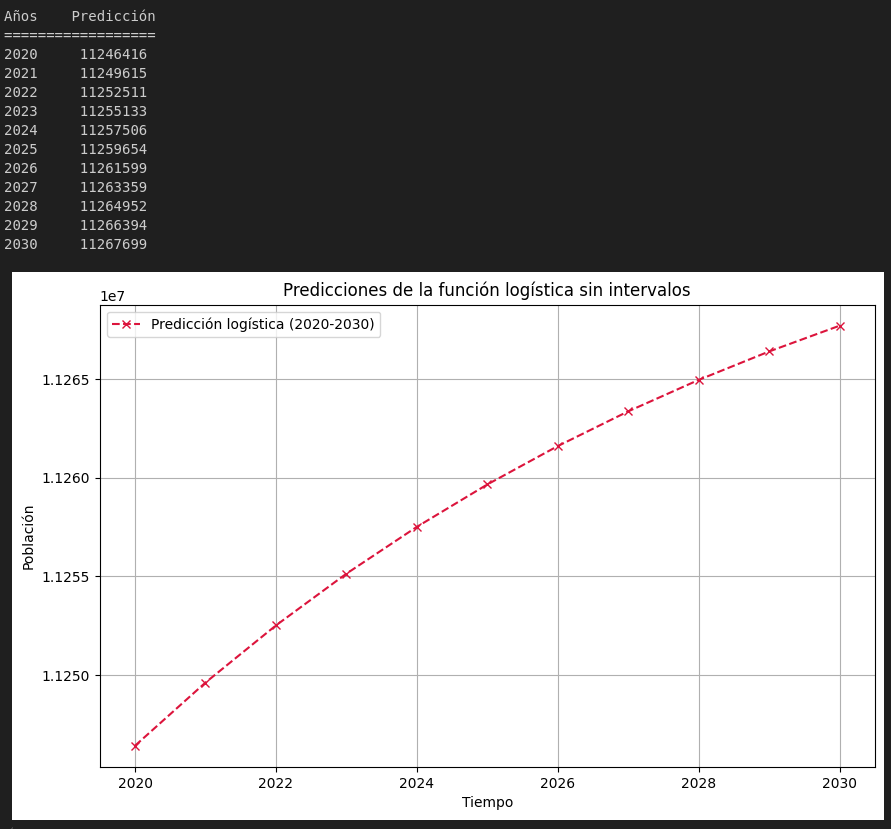
\includegraphics[width=0.45\textwidth]{img/graph_sin_intervalos.png}
\\
Por otro lado, como parte del modelo con intervalos se presentaron los siguientes resultados:\\
	\begin{figure}[h!]%
		\begin{center}
			\begin{tabular}{|c|c|c|} \hline
			 			& K 			& r 		\\ \hline
			0 			& 20442337054 	& 0.008  	\\ \hline
			1			& 340143106946 	& 0.003 	\\ \hline
			2			& 	  10660179	& -0.352 	\\ \hline
			3 			&   5105238279	&  0.000	\\ \hline
			4 			& 	2575174752	&  0.000 	\\ \hline
			5 			& 	   1223441	&  0.000	\\ \hline
			6 			& 	 999003076	&  0.000 	\\ \hline
			7 			& 	   1798999	&  0.000 	\\ \hline
			\end{tabular}
		\caption{Resultados del segundo modelo para el grupo de intervalos de 5 años \label{fig:ex}}
	\end{center}
\end{figure}
\\
En este caso fue donde el modelo tuvo peor ajuste, devolviendo unos valores ínfimamente menores a la existencia promedio y con una tasa nula. Esto se refleja visualmente si intentamos realizar una predicción con los parámetros del último intervalo:\\
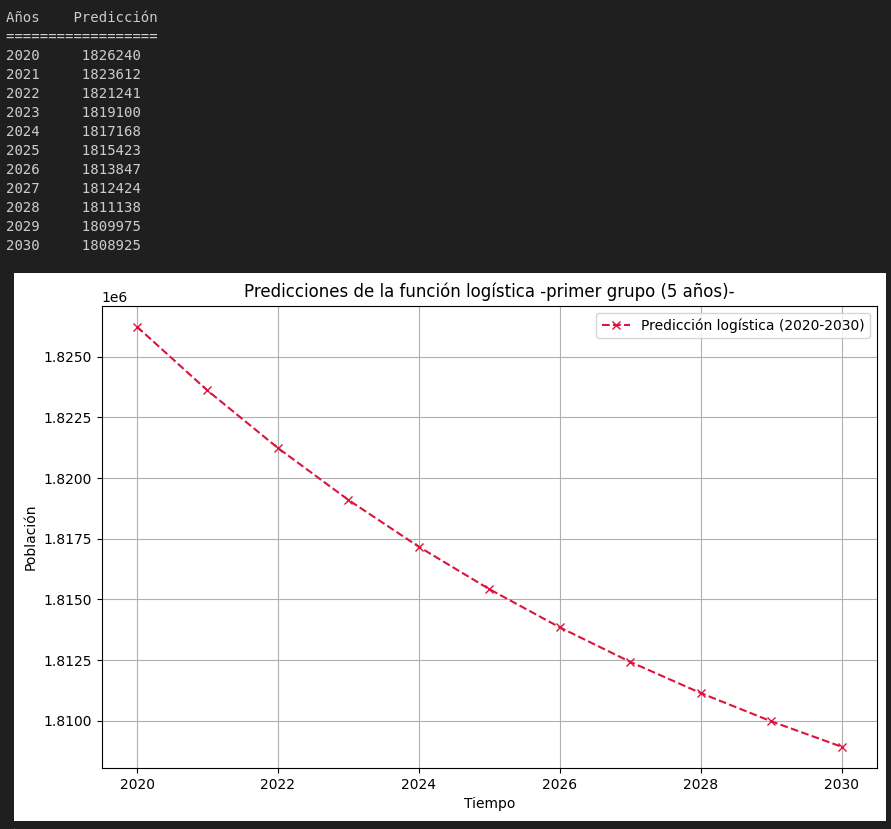
\includegraphics[width=0.45\textwidth]{img/df5_graph.png}
Obtenemos valores infimamente pequeños en comparación con la población media del pais.\\
Luego, para períodos de tiempo de 8 años:\\
\begin{figure}[h!]%
	\begin{center}
		\begin{tabular}{|c|c|c|} \hline
					 & K 			& r 		\\ \hline
			0		 & 2055969070415& 0.009		\\ \hline
			1		 & 10396071	    & -0.167	\\ \hline
			2		 & 10981262	    & -0.209	\\ \hline
			3		 & 1000853	    & 0.000		\\ \hline
			4		 & 11251162	    & 0.022		\\ \hline
		\end{tabular}
	\caption{Resultados del segundo modelo para el grupo de intervalos de 8 años \label{fig:ex}}
	\end{center}
\end{figure}
\\
Para este grupo se tuvieron los mejores resultados devolviendo en más de la mitad de los intervalos valores de $K$ y $r$ cercanos a la densidad poblacional promedio, como se puede observar gráficamente:
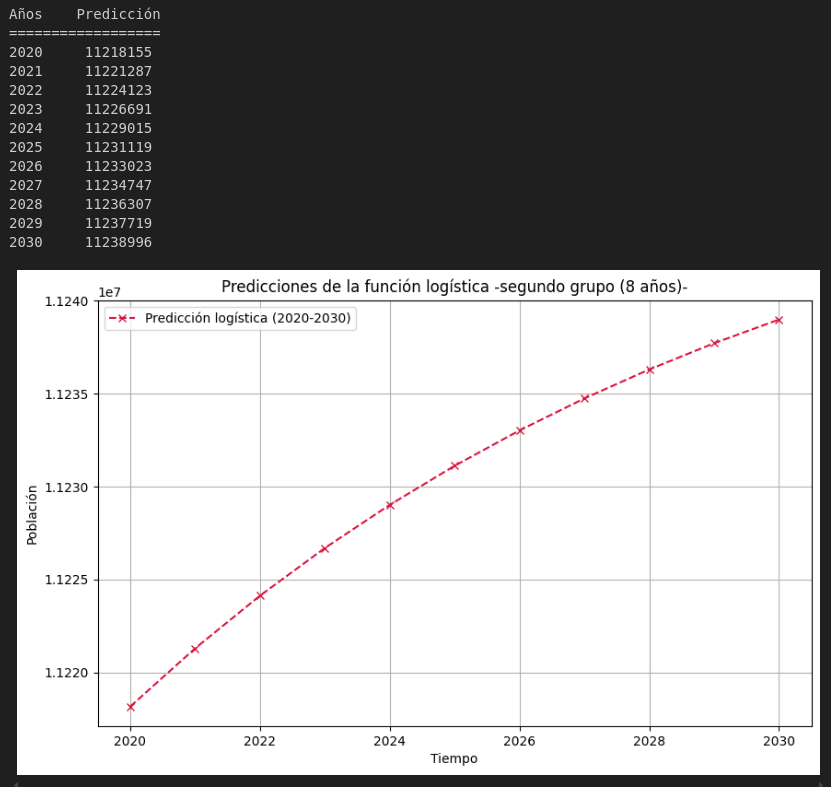
\includegraphics[width=0.45\textwidth]{img/df8_graph.png}
\\
Y finalmente, para grupos de 10 años:\\
\begin{figure}[h!]%
	\begin{center}
		\begin{tabular}{|c|c|c|} \hline
					 & K 			& r 		\\ \hline
			0		 & 2059434657188& 0.009		\\ \hline
			1		 &10623571		& -0.135	\\ \hline
			2		 & 726227		& -0.000	\\ \hline
			3		 & 5837330070	& 0.000		\\ \hline
		\end{tabular}
	\caption{Resultados del segundo modelo para el grupo de intervalos de 10 años \label{fig:ex}}
	\end{center}
\end{figure}
\\
Como última evaluación se tienen estos resultados, que, al igual que en el primer grupo, no se obtuvo un buen ajuste de los parámetros, en este caso para valores mosntruosamente mayores que la población media:
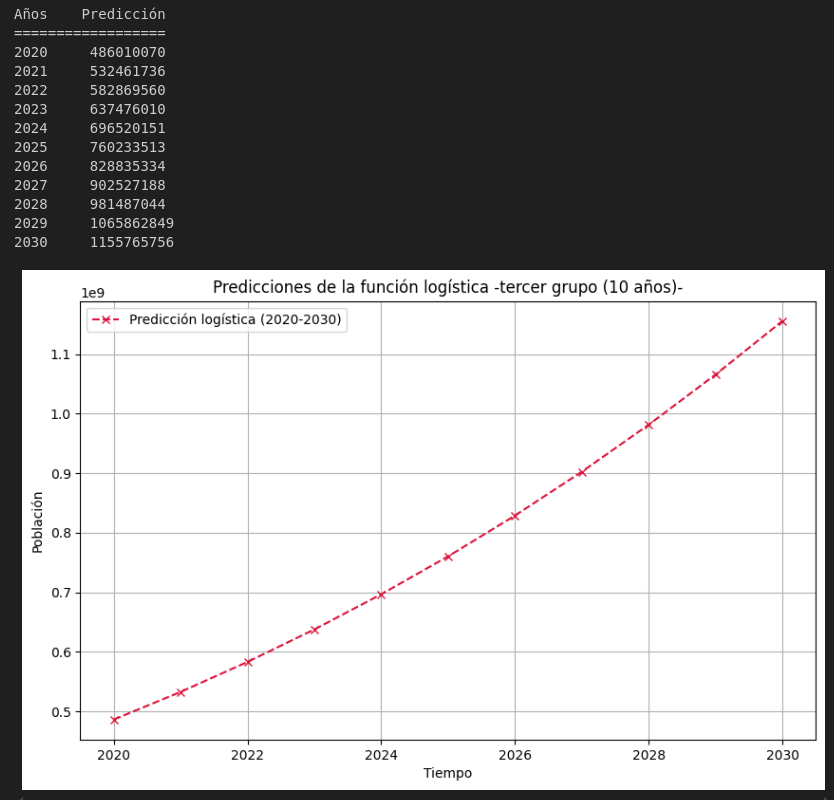
\includegraphics[width=0.45\textwidth]{img/df10_graph.png}
\\\\
Por tanto, de los resultados anteriores y de forma general con respecto al análisis se puede concluir:
\textbf{Impacto en K: }\\
La tendencia vertical observada en los datos puede afectar significativamente el valor de K. Teóricamente, cuando el tiempo tiende a infinito, la función poblacional tiende a K. Sin embargo, en la primera aproximación global, K proporcionó un valor cercano a la población total de Cuba (11 millones), lo cual sugiere que el modelo logístico tradicional no captura adecuadamente el comportamiento real de la población.\\
\textbf{Ajuste del Modelo:}\\
Dado que los datos reales no siguen exactamente la curva logística ideal, se propone un ajuste diferente al utilizado con todos los datos. Este nuevo ajuste se basaría en un crecimiento más acelerado, especialmente en los periodos donde se observa una tendencia más vertical. Esta modificación se justifica por los aumentos significativos en la población que se han registrado en esos momentos.\\
\textbf{Evaluación de Predicción:}\\
Los resultados de la evaluación de predicción mostraron que el segundo modelo (intervalos de 8 años) fue el que mejor se ajustó. Al representarlo, se reflejaron valores bastante cercanos a la densidad poblacional promedio, lo que indica un correcto ajuste del modelo.\\
\textbf{Crecimiento Poblacional en Cuba:}\\
En los años 1980 en adelante, Cuba experimentó un crecimiento poblacional significativo. Sin embargo, posteriormente se produjo un proceso de estabilización y eventual disminución de la tasa de crecimiento.

%===================================================================================

%===================================================================================
% Recomendaciones
%-----------------------------------------------------------------------------------
\section{Recomendaciones}\label{sec:rec}
\begin{itemize}
	\item Mejorar el Modelo Matemático:\\
-Desarrollar un modelo matemático más sofisticado que pueda capturar mejor la complejidad del crecimiento poblacional cubano. Esto podría incluir:\\
-Incorporar factores económicos, sociales y políticos que influyen en el crecimiento poblacional.\\
-Utilizar técnicas de modelado avanzadas, como modelos dinámicos o agentes, que puedan simular mejor la heterogeneidad temporal observada.\\
-Realizar un ajuste más preciso del modelo basado en el crecimiento acelerado observado en ciertos periodos. Esto podría implicar:\\
-Analizar en detalle los factores que causan los aumentos significativos en la población.\\
-Implementar un sistema de pesos diferentes para distintos periodos, dando mayor importancia a los segmentos de crecimiento más rápido.
	\item Ampliar la Base de Datos:\\ 
-Recopilar y analizar nuevos datos históricos que permitan una mejor comprensión del patrón de crecimiento poblacional en Cuba. Esto podría incluir:\\
-Información sobre migraciones internacionales y su impacto en la población.\\
-Datos detallados sobre la distribución geográfica de la población.\\
-Indicadores socio-económicos relacionados con el crecimiento poblacional.\\
-Integrar fuentes de información adicionales, como encuestas de salud pública o estudios demográficos nacionales, para obtener una visión más completa del fenómeno.
	\item Validar y Refinar el Modelo:\\ 
-Realizar pruebas de validación cruzada para evaluar la robustez del modelo frente a diferentes escenarios y condiciones.\\
-Comparar el rendimiento del modelo ajustado con el tradicional logístico, utilizando indicadores cuantitativos como la raíz cuadrática media (RMSE) o la correlación de Pearson.\\
-Realizar simulaciones prospectivas utilizando el modelo refinado para predecir el futuro crecimiento poblacional y compararlos con proyecciones oficiales.\\
	\item Investigar Factores Externos:\\ 
-Analizar el impacto de eventos macroeconómicos y geopolíticos en el crecimiento poblacional, como cambios en las relaciones internacionales de Cuba o reformas económicas.\\
-Estudiar cómo factores ambientales y climáticos podrían influir en el patrón de crecimiento poblacional, especialmente en un país insular como Cuba.
	\item Divulgar los Resultados:\\
-Presentar los hallazgos y recomendaciones en foros académicos y profesionales, buscando colaboraciones interdisciplinarias con economistas, sociólogos y científicos políticos.\\
-Sugirir aplicaciones prácticas de los resultados, como orientación para planificación urbana, desarrollo económico sostenible o formulación de políticas públicas.\\
Estas recomendaciones buscan fortalecer el modelo actual, ampliar su alcance y utilidad, y contribuir al conocimiento demográfico de Cuba, teniendo en cuenta las particularidades observadas en el análisis inicial.
\end{itemize}


%===================================================================================

%===================================================================================
% Bibliografía
%-----------------------------------------------------------------------------------
\begin{thebibliography}{99}
%-----------------------------------------------------------------------------------
	\bibitem{1} Los efectos y desafíos de la transformación demográfica en América latina y el Caribe. URL: \url{https://www.cepal.org/es/enfoques/efectos-desafios-la-transformacion-demografica-america-latina-caribe}.

	\bibitem{2} Wikipedia. URL: \url{https://es.wikipedia.org/wiki/Crecimiento_poblacional}

	\bibitem{3} Blog del Instituto de Matematicas de la Universidad de Sevilla. URL: \url{https://institucional.us.es/blogimus/2018/01/un-ejemplo-sencillo-de-modelizacion-matematica-el-crecimiento-de-poblaciones/}

	\bibitem{4} Openstax-Libro Calculo Volumen 2. URL: \url{https://openstax.org/books/c%C3%A1lculo-volumen-2/pages/4-4-la-ecuacion-logistica}
	
	\bibitem{5} Documentación Matplotlib. URL: \url{https://matplotlib.org/stable/index.html}.

	\bibitem{6} Datos históricos de crecimiento poblacional usados URL: \url{https://github.com/LFrench03/Modelo-de-Crecimiento-Poblacional/blob/main/data/csv/poblacion-residente.csv}

	\bibitem{7} Sitio web de la Oficia Nacional de Estadissticas e Informacion(ONEI) en la seccion de
	estadísticas demograficas. URL: \url{https://www.onei.gob.cu/}

	\bibitem{8} Documentación de SciPy. URL: \url{https://docs.scipy.org/doc/scipy/reference/generated/scipy.optimize.curve_fit.html}.

%-----------------------------------------------------------------------------------
\end{thebibliography}
\end{document}


